\section{Robotic Lawn Mowers}\label{roboMowers}
Several manufacturers of electrical gardening machines have started selling robotic lawn mowers in the recent years. In general they use one of these two strategies when cutting the lawn:
\begin{itemize}
	\item Random direction mowers
	\item Parallel line mowers
\end{itemize}
%
Mowers using the random direction strategy will drive in a straight line until a guard wire or an obstacle is detected. They will then turn in a random direction, and continue. See \figref{fig:randomcut}.

\begin{figure}[H]
\centering
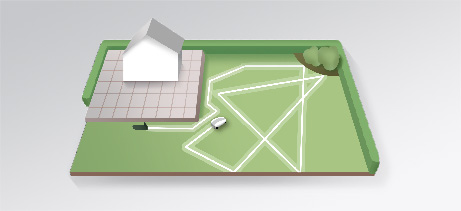
\includegraphics[scale=0.8]{figures/noLogiCut.jpg}
\caption{Random cut system [source:Bosch]} 
\label{fig:randomcut}
\end{figure}
\noindent
When the battery is nearly discharged, the mower will follow the guard wire back to the base station to recharge.\\\\
%
Parallel line mowers use a more intelligent control algorithm to optimize the mowing. After an initial learning run, following the guard wire around the lawn to be mowed, it will map the lawn, and cut in parallel lines, see \figref{fig:logicut}. The advantage of this strategy efficiency, is that the lawn mower will not run over the same spots more than once. According to Bosch, a given lawn can be mowed up to 30\% faster with their Logicut system \cite{Bosch}.

\begin{figure}[H]
\centering
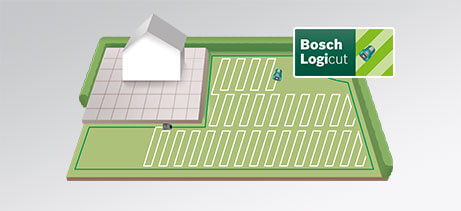
\includegraphics[scale=0.8]{figures/logicut.jpg} 
\caption{Bosch Logicut system [source:Bosch]}
\label{fig:logicut}
\end{figure}
\noindent

Common for both systems is the guard wire, which has to be placed around the lawn and anywhere the lawn mower is not allowed to go, like flower beds, swimming pools, etc. This technology choice in some existing robotic lawn mowers can be a problem.